\documentclass{article}
\setlength{\parskip}{5pt} % esp. entre párrafos
\setlength{\parindent}{0pt} % esp. al inicio de un párrafo
\usepackage{amsmath} % mates
\usepackage{url} % que las URLs se vean lindos
\usepackage[top=25mm,left=20mm,right=20mm,bottom=25mm]{geometry} % márgenes
\usepackage{parskip}
\usepackage[utf8]{inputenc}
\usepackage{amsmath,amsfonts,amssymb,mathtools}
\usepackage{graphicx,float}
\usepackage{algorithmic}
\usepackage{minted}
\usepackage{subcaption}
\usepackage{multicol}
\usepackage{listings}
\usepackage{xcolor}
\usepackage[sort&compress,numbers]{natbib} % referencias
\usepackage{minted}
\usepackage{hyperref} % ligas de URLs
\usepackage{graphicx} % poner figuras
\usepackage[spanish]{babel} % otros idiomas
\usepackage{listings}
\author{Raul L.} % author
\title{Pr\'{a}ctica 9: interacciones entre partículas} %título
\date{\today}
\begin{document} % inicia contenido

\maketitle % cabecera


\section{Introducci\'{o}n}\label{intro} % sección y etiqueta
En la novena práctica trabajamos con un modelo simplificado para los fenómenos de atracción y repulsión de física (o química, de hecho). Supongamos que contemos con $n$ partículas que habitan un cuadro unitario bidimensional y que cada partícula tiene una carga eléctrica, distribuida independientemente e normalmente al azar entre $[$-$1,1]$. Cargas de un mismo signo producirán una repulsión mientras cargas opuestas resultan en una atracción — la magnitud de la fuerza estará proporcional a la diferencia de magnitud de las cargas (mayores diferencias resultando en fuerzas mayores), y además la fuerza será inversamente proporcional a la distancia euclideana entre las partículas (éstas son reglas inventadas de interacción para efectos de demostración). Vamos a comenzar creando y posicionando las partículas, usando la distribución normal (posteriormente normalizada al cuadro unitario) para las coordenadas $x, y $ \citep{2}.


\section{Objetivo}
Agrega a cada partícula una masa y haz que la masa cause fuerzas gravitacionales (atracciones) además de las fuerzas causadas por las cargas. Estudia la distribución de velocidades de las partículas y verifica gráficamente que esté presente una relación entre los tres factores: la velocidad, la magnitud de la carga, y la masa de las partículas. Toma en cuenta que la velocidad también es afectada por las posiciones.\citep{2}.

\section{C\'{o}digo}
Para este código se utilizó como base el código de la doctora donde se hicieron modificaciones.

 Código en Python 

\url{https://github.com/satuelisa/Simulation/blob/master/Particles/creation.py}

{\bf Código creado en Python}

\url{https://github.com/Raullr28/Resultados/blob/main/P9/practica%20_9.py}

\renewcommand{\listingscaption}{Código}

\begin{listing}[H]
\begin{minted}{python}

paso = 256 // 10
niveles = [i/256 for i in range(0, 256, paso)]
colores = [(niveles[i], 0, niveles[-(i + 1)]) for i in range(len(niveles))]
palette = LinearSegmentedColormap.from_list('tonos', colores, N = len(colores))
 
from math import fabs, sqrt, floor, log
eps = 0.001
def fuerza(i, shared):
    p = shared.data
    n = shared.count
    pi = p.iloc[i]
    xi = pi.x
    yi = pi.y
    ci = pi.c
    mi = pi.m
    fx, fy = 0, 0
    for j in range(n):
        pj = p.iloc[j]
        cj = pj.c
        mj = pj.m
        dire = (-1)**(1 + (ci * cj < 0))
        dire_m = (-1)**(1 + (ci * cj < 0))
        dx = xi - pj.x
        dy = yi - pj.y
        factor = dire * fabs(ci - cj) / (sqrt(dx**2 + dy**2) + eps)
        factor_masa = dire_m * ((mi * mj) / ((sqrt(dx**2 + dy**2) + eps)))
        fx = fx - dx * factor * factor_masa
        fy = fy - dy * factor * factor_masa
    
    fx = fx
    fy = fy
    return (fx, fy)

  \end{minted}
  \label{lst:fibo}
  \caption{Representación de la función y parámetros utilizados.}
  
  
\end{listing}
\renewcommand{\listingscaption}{Código}
\begin{listing}[H]

\begin{minted}{python}
 

if __name__ == "__main__":
    n = 15
    x = np.random.normal(size = n)
    y = np.random.normal(size = n)
    c = np.random.normal(size = n)
    m = np.random.normal(size = n)
    xmax = max(x)
    xmin = min(x)
    x = (x - xmin) / (xmax - xmin) # de 0 a 1
    ymax = max(y)
    ymin = min(y)
    y = (y - ymin) / (ymax - ymin) 
    cmax = max(c)
    cmin = min(c)
    c = 2 * (c - cmin) / (cmax - cmin) - 1 # entre -1 y 1
    masamax = max(m)
    masamin = min(m)
    m = 5 * ((m - masamin) / (masamax - masamin) + 0.1)
    m = np.round(m).astype(int)
    g = np.round(5 * c).astype(int)
    vel = [[0]]*n
    p = pd.DataFrame({'x': x, 'y': y, 'm':m, 'c': c,'vel':vel,'g':g})

    x = p['x']
    y = p['y']
    c = p['c']
    m = p['m']
    g = p['g']

   
  \end{minted}
  \label{lst:fibo}
  \caption{Representación ciclo de la partícula.}
\end{listing}

%%%%%%%%%%%%%%%%%%%%% imagen 1
\begin{figure}[H]
\centering
\begin{subfigure}[b]{1.0\linewidth}
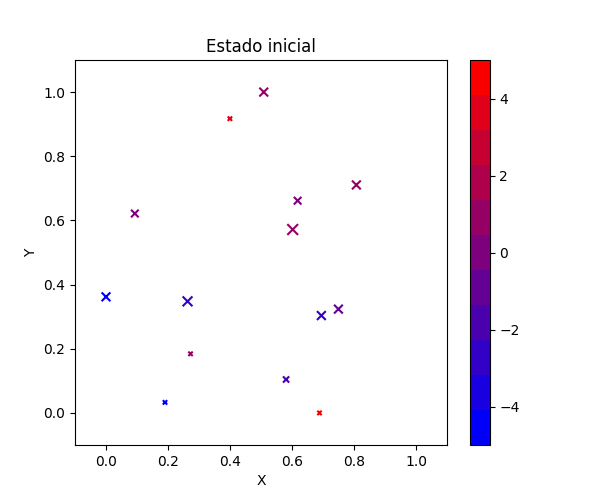
\includegraphics[width=\linewidth]{Imagenes/p9p_t0.png}
\end{subfigure}
\caption{Velocidad sobre tiempo de la partícula.}
\label{fig:westminster}
\end{figure}
%%%%%%%%%%%%%%%%%%%%%%%  final 


\newpage
% Computational Results
\section{Resultados}
En una gráfica de línea se graficó los resultados del comportamiento de las diferentes partículas respectivamente para poder ver su la importancia que toma al agregar el factor de la masa, como también se generaron caja bigotes para poder identificar el comportamiento en su velocidad y carga de la partícula.
%%%%%%%%%%%%%%%%%%%%% imagen 1
\begin{figure}[H]
\centering
\begin{subfigure}[b]{1.0\linewidth}
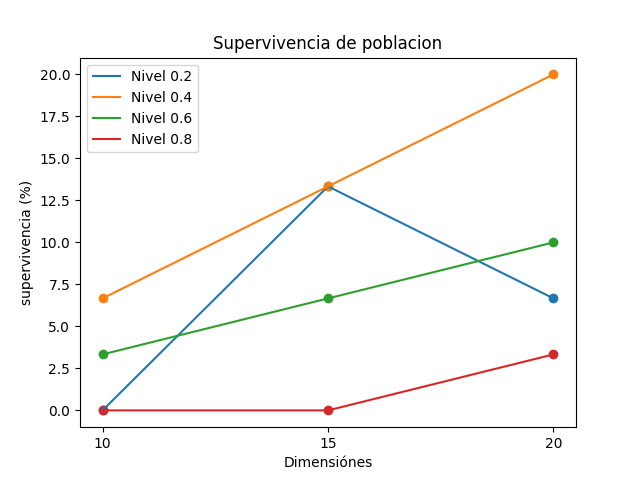
\includegraphics[width=\linewidth]{Imagenes/Figure_1.png}
\end{subfigure}
\caption{Velocidad sobre tiempo de la partícula.}
\label{fig:westminster}
\end{figure}
%%%%%%%%%%%%%%%%%%%%%%%  final 

%%%%%%%%%%%%%%%%%%%%% imagen 2
\begin{figure}[H]
\centering
\begin{subfigure}[b]{1.0\linewidth}
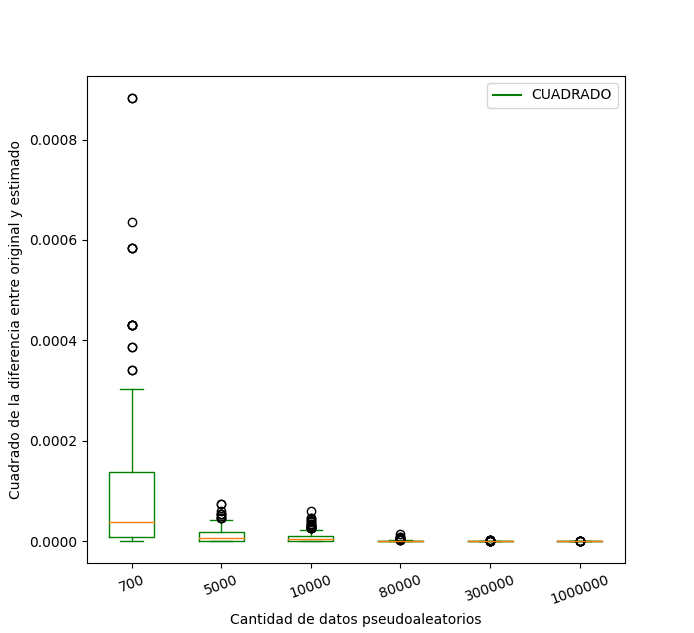
\includegraphics[width=\linewidth]{Imagenes/Figure_2.png}
\end{subfigure}
\caption{Velocidad sobre masa de la partícula.}
\label{fig:westminster}
\end{figure}
%%%%%%%%%%%%%%%%%%%%%%%  final 

%%%%%%%%%%%%%%%%%%%%% imagen 3
\begin{figure}[H]
\centering
\begin{subfigure}[b]{1.0\linewidth}
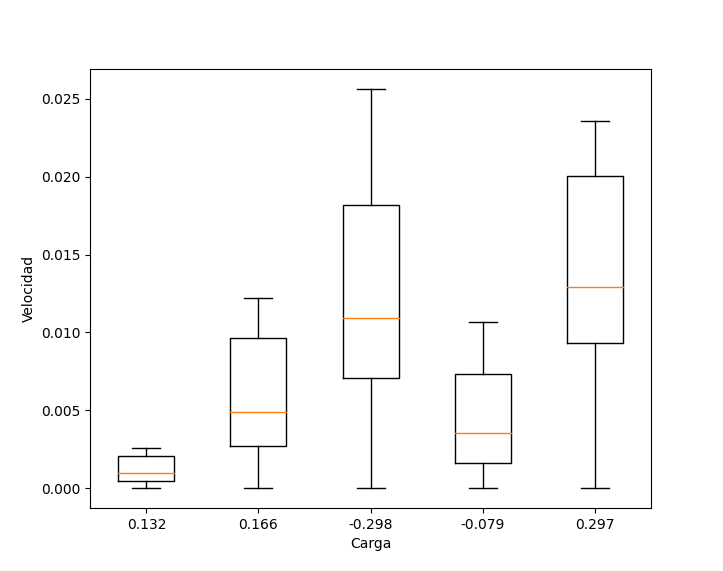
\includegraphics[width=\linewidth]{Imagenes/Figure_3.png}
\end{subfigure}
\caption{Velocidad sobre carga de la partícula.}
\label{fig:westminster}
\end{figure}
%%%%%%%%%%%%%%%%%%%%%%%  final 
\newpage
 \section{Conclusión}
Se mostró con gráficas de caja bigote que al tomar en cuenta la masa las partículas con más masa tienen hacer más positivas y a tener una mejor velocidad. 
.

 \bibliography{biblio.bib}
 \bibliographystyle{unsrtnat}

 \end{document}


